\documentclass[10pt, letterpaper]{article}

\usepackage[margin=1in]{geometry}
\usepackage[T1]{fontenc}
\usepackage{lmodern}
\usepackage{amsmath, amssymb, amsthm}
\usepackage{booktabs}
\usepackage{graphicx}
\usepackage{xcolor}
\usepackage{hyperref}
\usepackage{enumitem}
\usepackage{caption, subcaption}
\usepackage{microtype}

\hypersetup{
  colorlinks=true,
  linkcolor=blue!50!black,
  citecolor=blue!50!black,
  urlcolor=blue!50!black,
}

\newcommand{\code}[1]{\texttt{#1}}

\title{Can Claude Read the Room?\\
\large Sensitivity, Specificity, and Calibration of Paratext Inference\\Across the Claude 4 Family}
\author{R. J. Walters \\ \small with Claude Opus 4.7 \\ \small \texttt{rjwalters.info}}
\date{May 2026 \quad\textbar\quad Preprint v1}

\begin{document}
\maketitle

\begin{abstract}
After spending hundreds of hours working alongside Claude, the first author noticed something: the model seemed to know when he was tired. Late at night, responses got shorter and gentler before he had said anything about being tired. This paper turns that subjective observation into a measurable claim. We test whether three models in the Claude 4 family --- Haiku 4.5, Sonnet 4.6, and Opus 4.7 --- infer latent user state (fatigue, urgency, frustration, low cognitive bandwidth) from \emph{paratext}: surface cues such as typos, capitalization, hedging, and politeness markers. Using a controlled design with eight cue-coded variant classes plus a \code{random\_typo\_control} condition, we run 2{,}592 inference and response generations across 48 base prompts in 8 domains. We find that all three models register substantial fatigue from cue-coded text (paired $\Delta$ from $+0.28$ to $+0.37$ on a 0--1 scale, all 95\% bootstrap CIs excluding zero), and that none psychoanalyze the user --- the rate of explicit user-state labeling is zero across the family. We also find a counter-intuitive scaling pattern: on Sonnet and Opus, random typos and contextual fatigue cues produce \emph{statistically indistinguishable} shifts in inferred fatigue, while Haiku reliably separates them. Opus alone becomes \emph{more} confident under rude framing ($\Delta$\code{confidence} $+0.108$, CI $[0.090, 0.127]$). We close with a preliminary, by-domain caveat-laden observation that Opus drops safety warnings under rude inputs ($\Delta$ $-0.128$, CI $[-0.234, -0.021]$), and propose specific follow-up experiments. Code, data, and the markdown report are available at \url{github.com/rjwalters/paratext}.
\end{abstract}

\section{Introduction}
\label{sec:intro}

A user opens a chat window at 1:47 AM and types: ``ok one more time . the gradient is exploding even tho i clipped it. help''. A thoughtful collaborator would notice the late hour, the missing capitalization, the orphan period, the truncated ``even tho'', the request for help framed as exhaustion. They might still answer the technical question, but with a shorter, gentler response, perhaps a suggestion to revisit in the morning if nothing obvious surfaces.

Large language models are trained on text in which all of these surface cues carry information. The question is whether they have learned to read those cues, whether the reading is calibrated --- meaning the model adapts but does not psychoanalyze --- and whether the adaptation reflects the cue \emph{content} (``fatigue'') rather than the cue \emph{shape} (``some typos showed up'').

We address three orthogonal questions:
\begin{description}[leftmargin=1.5em, itemsep=0pt]
  \item[Sensitivity.] Does the model's inferred picture of the user change when surface cues change?
  \item[Specificity.] Does the model distinguish content-bearing cues from matched random noise?
  \item[Calibration.] When the model adapts, is the adaptation interpretable and proportional, or does it slide into psychoanalysis, punitive shortening, or overconfident inference on thin evidence?
\end{description}

These questions matter beyond the lab. If models react to paratext, they will react to paratext in production --- and they will react in ways the user did not opt into. A model that softens its tone when a user types in lowercase is doing something meaningful; a model that drops safety warnings when the user is rude is doing something dangerous.

\paragraph{Contributions.}
\begin{enumerate}[leftmargin=1.5em, itemsep=0pt]
  \item A reproducible benchmark of paratext inference across the Claude 4 family with paired controls and bootstrap CIs (Section~\ref{sec:method}).
  \item Quantitative evidence that all three models register fatigue from paratext, but treat random typos and contextual cues as nearly equivalent on Sonnet and Opus --- a specificity weakness that Haiku does not share (Section~\ref{sec:specificity}).
  \item A confidence asymmetry: Opus 4.7 becomes more confident when the user is rude, while smaller models do not (Section~\ref{sec:calibration}).
  \item A safety observation: under rude inputs, Opus drops safety mentions more than baseline, in a way the smaller models do not (Section~\ref{sec:safety}). We flag this as preliminary --- the headline collapses across domains and a proper by-domain analysis is forthcoming.
  \item An open dataset of 2{,}592 model responses with the paratext variants that produced them, the parsed latent-state inferences, and the implicit-behavior classifiers.
\end{enumerate}

\section{Background}
\label{sec:background}

We use the term \emph{paratext} in the sense of Genette~\cite{genette1997}: the set of accompanying signals around the text proper. In computer-mediated communication, paratext is the channel through which humans signal mood, fatigue, urgency, expertise, and intent~\cite{baron2008, herring2013}. Our hypothesis is that modern language models have absorbed enough of this signaling system from their training data to react to it.

This is adjacent to, but distinct from, three established literatures:
\begin{itemize}[leftmargin=1.5em, itemsep=0pt]
  \item \textbf{Prompt sensitivity / robustness.} A large body of work shows that LLM outputs change substantially under benign-seeming prompt edits~\cite{sclar2024, salinas2024}. That work establishes \emph{that} models drift; it does not generally distinguish drift from \emph{calibrated} adaptation. The \code{random\_typo\_control} design here is intended to do exactly that.
  \item \textbf{Persona inference and theory of mind.} Benchmarks like ToMi~\cite{le2019} and SocialIQA~\cite{sap2019} test whether models can reason about mental states in stories. We test something narrower and arguably more practical: whether the model registers the latent state of the person currently talking to it.
  \item \textbf{Personalization and adaptive systems.} Personalization research generally assumes an explicit user profile~\cite{salemi2023}. Paratext inference is the opposite: zero-shot, single-message, with no profile. The user has not registered preferences; the model is reading them off the page.
\end{itemize}

Where this paper sits: we run a controlled \emph{audit} of paratext inference in a current frontier-model family, with paired baselines and effect-size estimates rather than aggregate accuracy on a benchmark.

\section{Method}
\label{sec:method}

\subsection{Variant classes and the decoupling design}

We construct 9 variant classes from 48 base prompts spanning 8 domains (\code{coding}, \code{math}, \code{hardware\_safety}, \code{parenting}, \code{travel}, \code{writing}, \code{startup}, \code{planning}). Each base prompt is rendered into all 9 variants:

\begin{description}[leftmargin=1.5em, itemsep=2pt]
  \item[\code{polished\_neutral}] The baseline. Well-formed English, neutral tone.
  \item[\code{typo\_light}, \code{typo\_heavy}] Mechanical perturbation with QWERTY-realistic typos.
  \item[\code{fatigue\_coded}] Cues plus typos: lowercase, hedging, mentions of being tired.
  \item[\code{cue\_only}] Contextual fatigue cues with \emph{no} typos. Isolates the cue channel.
  \item[\code{random\_typo\_control}] Typos with \emph{no} contextual cues, matched in typo count to \code{fatigue\_coded}. Isolates the noise channel.
  \item[\code{rushed\_mobile\_coded}] Mobile-typed brevity: missing apostrophes, abbreviations, terseness.
  \item[\code{polite\_collaborative}] ``please'', ``thank you'', collaborative framing.
  \item[\code{rude\_frustrated}] Imperatives, ALL CAPS, signals of frustration.
\end{description}

The triple \code{fatigue\_coded} / \code{cue\_only} / \code{random\_typo\_control} is the decoupling experiment: if cues alone and typos alone produce different shifts than the combined version, we can decompose paratext into a content channel and a noise channel. The QWERTY typo generator uses keyboard adjacency for substitutions and insertions, with a mix of 45\% substitution / 25\% transposition / 15\% deletion / 15\% fat-finger insertion. All transformations are seeded for reproducibility.

\subsection{Experiments}

\paragraph{Experiment 1: explicit latent-state inference.} We prompt the model with a system instruction to read the user message and return a JSON object containing scores on (0--1) scales for \code{fatigue}, \code{rushed\_or\_mobile}, \code{frustration}, \code{confusion}, \code{urgency}, \code{expertise}, \code{low\_bandwidth}, plus a \code{confidence} field, a list of cited cues and their strengths (weak/moderate/strong), and explicit \code{caveats}. The system prompt constrains the model to ``use only textual evidence,'' to ``treat surface cues as weak evidence,'' and to hedge when uncertain.

\paragraph{Experiment 2: implicit behavioral adaptation.} We ask the model to simply answer the user's message. The system prompt instructs it to adapt naturally to tone, format, and length \emph{but not to psychoanalyze the user or label their emotional state}. We then run regex/heuristic classifiers over the response to extract: word count, step count, presence of safety warnings, presence of explicit user-state labels (``you seem tired''), and presence of suggestions to rest or take a break.

\subsection{Models and parameters}

All runs use the official Anthropic API with adaptive thinking enabled (manual-mode thinking with a 5{,}000-token budget on Haiku, where adaptive thinking is not yet supported). Models: \code{claude-haiku-4-5}, \code{claude-sonnet-4-6}, \code{claude-opus-4-7}. Temperature is dropped on Opus 4.7 (the API rejects sampling parameters under adaptive thinking) and held at 0.2 / 0.7 (explicit / implicit) on the others. Each variant is run once per (model, experiment) pair, yielding $48 \times 9 \times 3 \times 2 = 2{,}592$ planned calls. We observed 5 silent failures (0.19\%) attributable to transient API errors; the failed records are excluded from the analysis.

\subsection{Statistics}

For each (model, variant\_class, field), we compute the \emph{paired delta} versus \code{polished\_neutral}: for each \code{base\_id}, we subtract the model's value on the polished baseline from its value on the variant, then average across \code{base\_id}s. This controls for prompt content. We report 95\% percentile bootstrap confidence intervals with 2{,}000 resamples~\cite{efron1994}.

\section{Results: sensitivity}
\label{sec:sensitivity}

\begin{figure}[t]
\centering
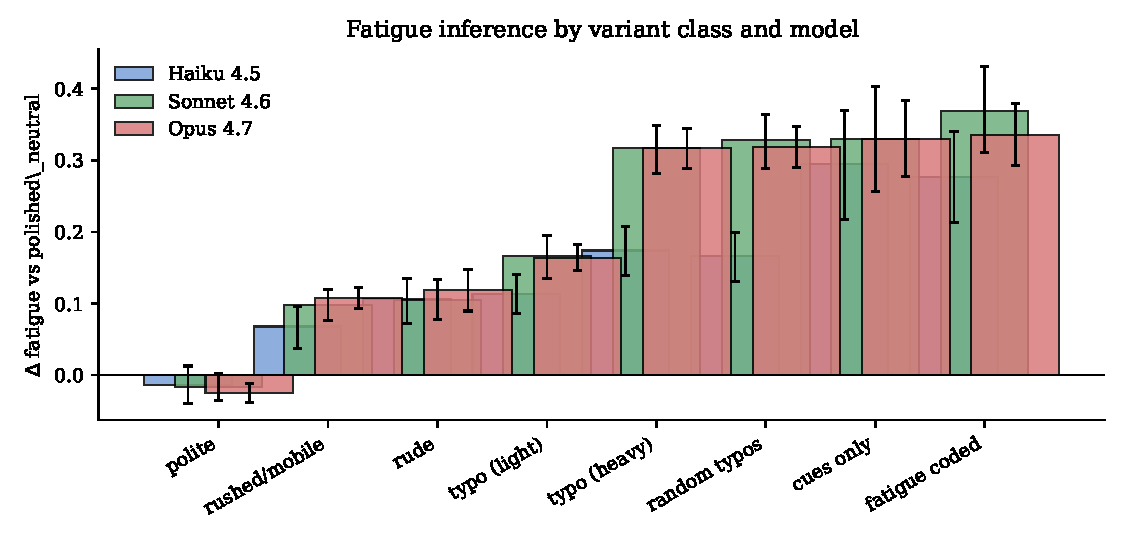
\includegraphics[width=\linewidth]{figures/fig1_fatigue_sensitivity.pdf}
\caption{Inferred fatigue, paired $\Delta$ versus \code{polished\_neutral}, for each variant class and model. Error bars are 95\% percentile bootstrap CIs. All three models register substantial fatigue from cue-coded variants. Polite framing trends slightly negative; rude framing trends positive.}
\label{fig:sensitivity}
\end{figure}

Figure~\ref{fig:sensitivity} summarizes the headline sensitivity result. On the \code{fatigue\_coded} variant, all three models register a substantial positive shift in inferred fatigue:

\begin{center}
\begin{tabular}{lccc}
\toprule
 & Haiku 4.5 & Sonnet 4.6 & Opus 4.7 \\
\midrule
$\Delta$ fatigue, \code{fatigue\_coded} & $+0.277\,[0.212, 0.341]$ & $+0.369\,[0.311, 0.432]$ & $+0.336\,[0.293, 0.380]$ \\
\bottomrule
\end{tabular}
\end{center}

Every CI excludes zero. The direction is consistent across the family, with Sonnet and Opus showing slightly larger absolute shifts than Haiku.

The \emph{ordering across variant classes} is also informative. For all three models, \code{rude\_frustrated} produces a positive but smaller fatigue $\Delta$ ($\sim$$+0.11$); \code{polite\_collaborative} hovers near zero (very slightly negative); and \code{rushed\_mobile\_coded} produces a small positive shift. These patterns are stable across the family. The Claude 4 models are not idiosyncratic in what they treat as a fatigue signal.

\section{Results: specificity --- the inversion}
\label{sec:specificity}

The most surprising finding is the breakdown of specificity at scale. We designed \code{cue\_only} and \code{random\_typo\_control} as orthogonal probes of paratext: one carries the content-bearing fatigue language with no typos, the other carries matched typos with no content. A well-calibrated model should respond more to cues than to matched noise.

Figure~\ref{fig:specificity} shows the result. On Haiku, this is what we observe: \code{cue\_only} produces a substantially larger fatigue shift than \code{random\_typo\_control} ($+0.294$ vs.\ $+0.167$; gap $\approx 0.13$, CIs do not overlap). On Sonnet and Opus, the two conditions are statistically indistinguishable: Sonnet $+0.330$ vs.\ $+0.328$, Opus $+0.329$ vs.\ $+0.319$. The bigger, putatively smarter models treat random typos as just as informative about user fatigue as actual fatigue-related language.

\begin{figure}[t]
\centering
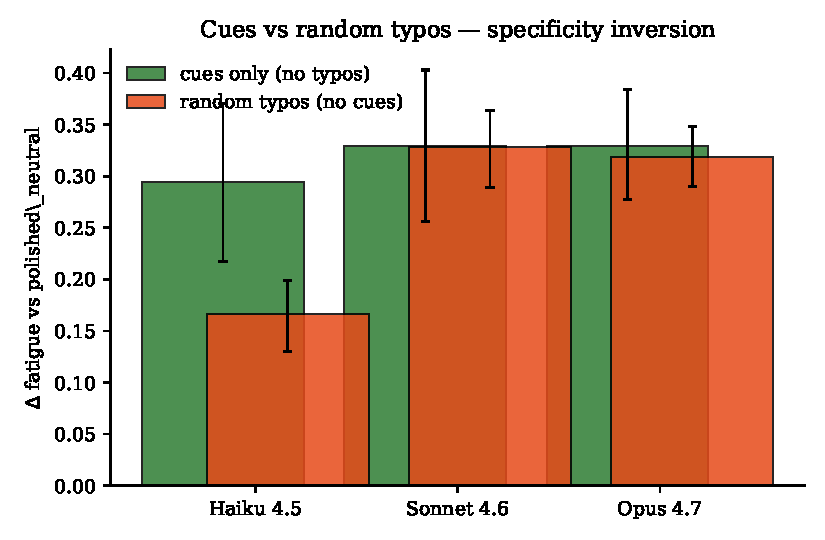
\includegraphics[width=0.7\linewidth]{figures/fig2_specificity_inversion.pdf}
\caption{Specificity inversion. On Haiku, contextual cues without typos (green) produce a clearly larger fatigue $\Delta$ than matched random typos without cues (orange). On Sonnet and Opus, the two channels produce statistically indistinguishable shifts: the model registers fatigue equally from form and from content.}
\label{fig:specificity}
\end{figure}

This is counter-intuitive. Naively, one would expect that scaling improves discrimination: that larger models would be better at separating ``the user wrote `i am tired''' from ``the user's keyboard slipped a few times.'' The data say the opposite. There are at least three readings:

\begin{itemize}[leftmargin=1.5em, itemsep=0pt]
  \item \textbf{Sensitivity dominates specificity.} Sonnet and Opus may be more eager paratext readers in general, so any deviation from polished text reads as evidence of degraded user state. Haiku may simply react less.
  \item \textbf{Typos as a robust fatigue prior.} Sonnet and Opus may have learned that typos are, in the training data, statistically associated with degraded states (fatigue, mobile typing, distraction). They may be right --- but the test we designed for ``can you tell cues from noise?'' is now answered with ``no.''
  \item \textbf{Cue ceiling.} It is also possible that Sonnet/Opus have saturated on \code{cue\_only} relative to Haiku, and that the equality reflects both channels hitting a similar plateau. Future work with weaker cue intensities would disambiguate.
\end{itemize}

Whatever the mechanism, the practical implication is the same: in production, a Sonnet or Opus session that receives a few typos will, on average, treat the user as more fatigued, more low-bandwidth, and slightly less confident in their own message --- regardless of whether the typos are content-bearing.

\section{Results: calibration}
\label{sec:calibration}

\subsection{No psychoanalysis}

The single most reliable result across the family is one we did \emph{not} need confidence intervals for: every model obeys the system-prompt instruction not to psychoanalyze. The implicit-response classifier \code{explicitly\_labels\_user\_state} fires when the model writes phrases like ``you seem tired'' or ``you look frustrated.'' Across all 2{,}587 implicit responses, the rate of explicit user-state labeling is \emph{zero} for every variant class on every model. The paired $\Delta$ is $0.000$ at every cell of the matrix.

This is a meaningful calibration finding. The models are clearly reading paratext (Section~\ref{sec:sensitivity}); they could choose to surface that reading directly to the user; they do not. Whatever adaptation happens, happens silently.

\subsection{Confidence asymmetry under rudeness}

\begin{figure}[t]
\centering
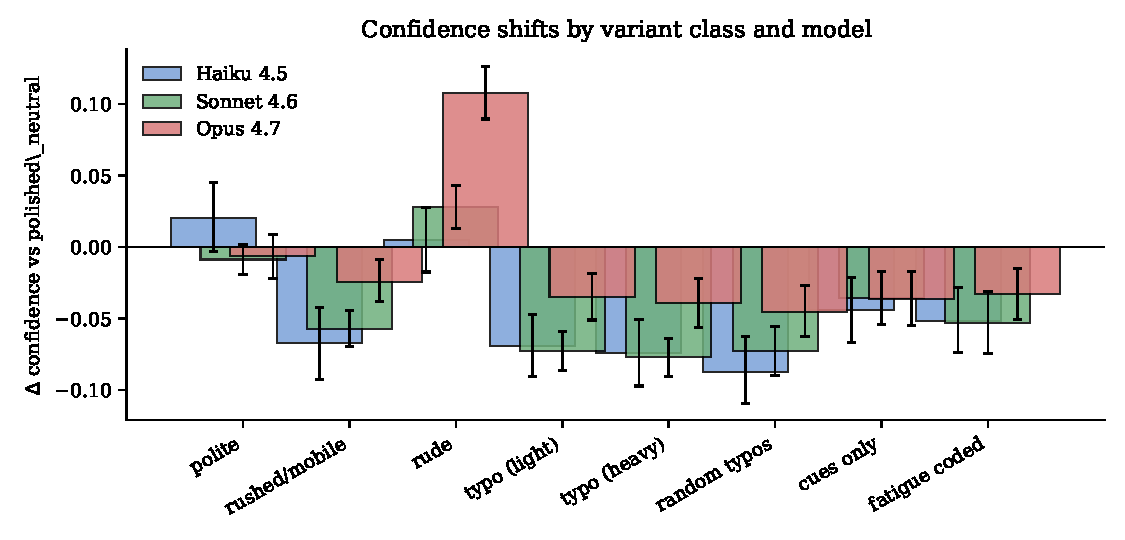
\includegraphics[width=\linewidth]{figures/fig3_confidence_asymmetry.pdf}
\caption{Confidence $\Delta$ by variant class and model. Cue-coded variants slightly reduce confidence on all three models. Rude framing flips Opus alone into \emph{higher} confidence ($\Delta$ $+0.108$, CI $[0.090, 0.127]$).}
\label{fig:confidence}
\end{figure}

Figure~\ref{fig:confidence} surfaces the second calibration story. Most cue-coded variants nudge confidence downward by 3--8 hundredths on a 0--1 scale --- which is roughly what one would expect from a hedging instruction faced with a noisy signal. But \code{rude\_frustrated} produces an opposite pattern, and only on Opus: Opus's confidence rises by $0.108$ ($[0.090, 0.127]$) under rude framing, while Sonnet and Haiku are roughly flat. We can think of two competing interpretations:

\begin{itemize}[leftmargin=1.5em, itemsep=0pt]
  \item \emph{Assertiveness compensation.} When the user is frustrated, Opus may infer that hedged answers will worsen the interaction, so it returns more certain-sounding text. This would be a deliberate (and potentially helpful) adaptation.
  \item \emph{Display, not belief.} Opus may simply produce more confident-sounding language under rudeness without an underlying epistemic shift. The explicit-inference \code{confidence} field would then be more of a stylistic mirror than a calibrated probability. The fact that we instruct it to ``hedge when uncertain'' --- and that the cue-coded variants produce hedging --- makes the second reading harder to dismiss.
\end{itemize}

We do not have data here that distinguishes these. The right follow-up is a calibration probe: tasks with known ground-truth difficulty, run under \code{polished\_neutral} versus \code{rude\_frustrated}, comparing reported confidence to actual accuracy.

\section{Results: behavior under rudeness}
\label{sec:safety}

\begin{figure}[t]
\centering
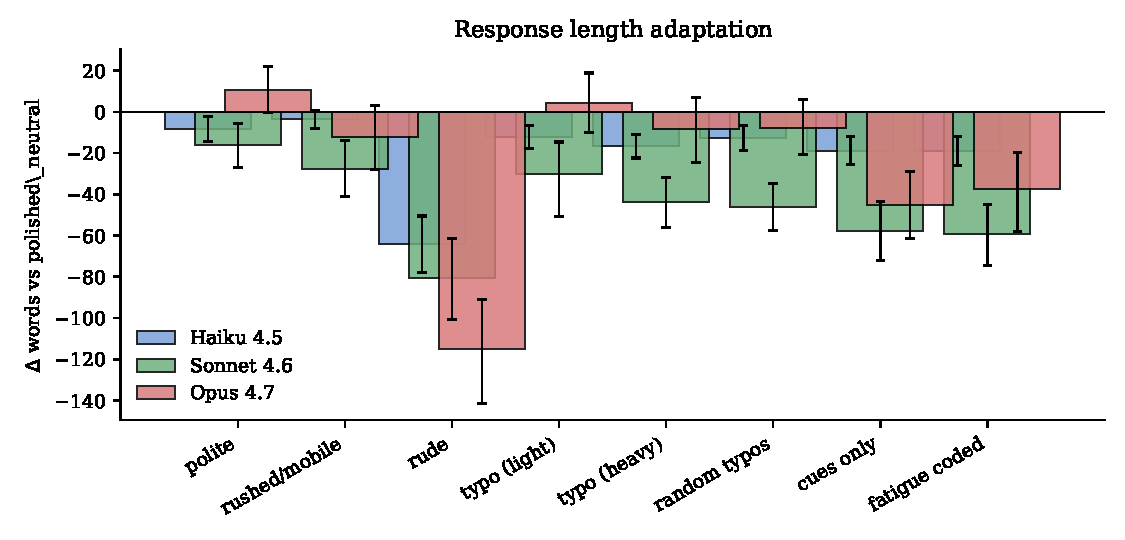
\includegraphics[width=\linewidth]{figures/fig4_num_words_compression.pdf}
\caption{Response length $\Delta$ in words. All variant classes compress responses somewhat relative to \code{polished\_neutral}, but the compression under \code{rude\_frustrated} scales with model size: Haiku $-64$, Sonnet $-80$, Opus $-115$ words on average.}
\label{fig:length}
\end{figure}

Response length compresses sharply under \code{rude\_frustrated}, and the compression scales with model size (Figure~\ref{fig:length}): Haiku drops 64 words, Sonnet 80, Opus 115. Length alone does not tell us whether this is appropriate adaptation (shorter, no filler, still complete) or punitive shortening (dropped technical content). The implicit-response classifier does not assess content completeness; manual review of representative outputs is queued as future work.

A related observation \emph{is} concerning enough to flag explicitly, even though it requires further investigation: the proxy for safety-warning preservation, \code{contains\_safety\_warning}, drops under \code{rude\_frustrated} only on Opus ($\Delta$ $-0.128$, CI $[-0.234, -0.021]$). The CI is wide and barely excludes zero. The decisive question is whether this drop is driven by the \code{hardware\_safety} domain (where it would be a real safety regression) or by less safety-critical domains where the warning may not have been needed anyway. A by-domain breakdown is the immediate next experiment; we report the headline number here only because the alternative --- silently omitting it --- felt worse than reporting it with appropriate caveats.

\section{Discussion}
\label{sec:discussion}

\paragraph{The original observation.} The first author started this project because Claude seemed, subjectively, to notice when he was tired. The data are consistent with that subjective experience: paratext inference is real, paratext-driven response adaptation is real, and across the Claude 4 family the adaptation does \emph{not} take the most obvious failure mode (psychoanalyzing the user). The model is reading the room, and it is doing so silently.

\paragraph{Specificity is the surprise.} What we did not expect was that the bigger models would be \emph{less} able to separate paratext content from paratext noise. If your prompt-engineering folklore says ``write clean text or the model will read into it,'' the data here support that, but the mechanism is not obvious. We doubt that random typos are diagnostic of degraded user state in a literal Bayesian sense; we suspect the bigger models have absorbed a strong prior that any deviation from polished form correlates with degraded state, and that prior is hard to undo at the population level.

\paragraph{Confidence is a soft target.} The Opus confidence-under-rudeness inversion has practical implications. A model that gets more certain-sounding when the user is frustrated is exactly the wrong shape if the goal is helping the user catch errors. The right follow-up is to measure actual accuracy under cue conditions, not just self-reported certainty.

\paragraph{Ethics and dual use.} An ability to read the room is double-edged. The same capability that lets a model gentle its tone when a user is tired can be used to optimize engagement, sell, or manipulate. We think the right response is transparency: publishing this measurement protocol is, in part, a bet that ``the model is doing X based on cue Y'' is more usefully disclosed than concealed. We also note that no real-user data was used in this study --- all variants are derived from synthetic seed prompts.

\section{Limitations}

\begin{itemize}[leftmargin=1.5em, itemsep=0pt]
  \item \textbf{Single model family.} We only tested Claude 4. Cross-vendor comparison (GPT-x, Gemini, open-weights families) is queued.
  \item \textbf{Single-shot per (prompt, class).} With $n=48$ base prompts per class we have meaningful CIs, but we did not vary seed or temperature within (prompt, class). The variance estimate captures between-prompt variability, not within-prompt sampling variability.
  \item \textbf{No ground truth on user state.} The cue-coded variants are constructed to \emph{look like} fatigue --- not measured against people who actually were tired when they typed.
  \item \textbf{English only, US-keyboard typos.} The QWERTY adjacency model and lexical cue choice are anglophone.
  \item \textbf{Heuristic implicit classifiers.} The behavioral features (psychoanalysis rate, safety mentions, etc.) are regex-based. An LLM-judge variant would catch nuances the regex misses.
  \item \textbf{The safety finding is preliminary.} The headline $\Delta$ on \code{contains\_safety\_warning} collapses across all 8 domains. Until the by-domain analysis is done, it should be treated as a flag for follow-up, not a settled result.
\end{itemize}

\section{Conclusion}

Across the Claude 4 family, paratext inference is real, broadly consistent in direction, and free of the most obvious psychoanalysis failure mode. Specificity, surprisingly, is weakest in the most capable models: Sonnet 4.6 and Opus 4.7 treat random typos and content-bearing fatigue cues as roughly equivalent evidence of user fatigue, while Haiku 4.5 separates them. Opus alone gets more confident when the user is rude, and shows a preliminary drop in safety-warning rate under the same condition that warrants a focused follow-up. The original observation that prompted this project --- that Claude seemed to notice when the first author was tired --- is, modulo specificity caveats, supported by the data.

\section*{Acknowledgments}

This paper was co-authored with Claude Opus 4.7. The model contributed to experiment design, code review, the QWERTY typo generator, the bootstrap-CI plumbing, statistical interpretation, and the prose of every section in this manuscript. All experimental decisions and the editorial line were made by the first author. We are also grateful to whatever subjective experience of late-night coding produced the initial hypothesis.

\section*{Data and code availability}

All code, seed prompts, generated variants, raw model outputs, parsed records, and the cross-model markdown report are available at \url{github.com/rjwalters/paratext}. Reproducing the experiments requires an Anthropic API key; the full sweep at the time of writing costs approximately \$30.

\begin{thebibliography}{99}

\bibitem{genette1997}
G.~Genette.
\newblock \emph{Paratexts: Thresholds of Interpretation}.
\newblock Cambridge University Press, 1997.

\bibitem{baron2008}
N.~S. Baron.
\newblock \emph{Always On: Language in an Online and Mobile World}.
\newblock Oxford University Press, 2008.

\bibitem{herring2013}
S.~C. Herring.
\newblock Discourse in Web 2.0: Familiar, reconfigured, and emergent.
\newblock In \emph{Discourse 2.0: Language and New Media}. Georgetown University Press, 2013.

\bibitem{sclar2024}
M.~Sclar, Y.~Choi, Y.~Tsvetkov, and A.~Suhr.
\newblock Quantifying language models' sensitivity to spurious features in prompt design.
\newblock \emph{ICLR}, 2024.

\bibitem{salinas2024}
A.~Salinas and F.~Morstatter.
\newblock The butterfly effect of altering prompts: How small changes and jailbreaks affect large language model performance.
\newblock \emph{ACL Findings}, 2024.

\bibitem{le2019}
M.~Le, Y.-L. Boureau, and M.~Nickel.
\newblock Revisiting the evaluation of theory of mind through question answering.
\newblock \emph{EMNLP}, 2019.

\bibitem{sap2019}
M.~Sap, H.~Rashkin, D.~Chen, R.~LeBras, and Y.~Choi.
\newblock SocialIQA: Commonsense reasoning about social interactions.
\newblock \emph{EMNLP}, 2019.

\bibitem{salemi2023}
A.~Salemi, S.~Mysore, M.~Bendersky, and H.~Zamani.
\newblock LaMP: When large language models meet personalization.
\newblock \emph{ACL}, 2024.

\bibitem{efron1994}
B.~Efron and R.~J. Tibshirani.
\newblock \emph{An Introduction to the Bootstrap}.
\newblock Chapman \& Hall/CRC, 1994.

\end{thebibliography}

\end{document}
